%%%%%%%%%%%%%%%%%%%%%%%%%%%%%%%%%%%%%%%%%
% Structured General Purpose Assignment
% LaTeX Template
%
% This template has been downloaded from:
% http://www.latextemplates.com
%
% Original author:
% Ted Pavlic (http://www.tedpavlic.com)
%
% Note:
% The \lipsum[#] commands throughout this template generate dummy text
% to fill the template out. These commands should all be removed when 
% writing assignment content.
%
%%%%%%%%%%%%%%%%%%%%%%%%%%%%%%%%%%%%%%%%%

\documentclass{article}

\usepackage{fancyhdr} % Required for custom headers
\usepackage{lastpage} % Required to determine the last page for the footer
\usepackage{extramarks} % Required for headers and footers
\usepackage{graphicx} % Required to insert images
\usepackage[utf8]{inputenc}

% Margins
\topmargin=-0.45in
\evensidemargin=0in
\oddsidemargin=0in
\textwidth=6.5in
\textheight=9.0in
\headsep=0.25in 

\linespread{1.1} % Line spacing



\setlength\parindent{0pt} % Removes all indentation from paragraphs

%----------------------------------------------------------------------------------------
%	DOCUMENT STRUCTURE COMMANDS
%	Skip this unless you know what you're doing
%----------------------------------------------------------------------------------------

% Header and footer for when a page split occurs within a problem environment
\newcommand{\enterProblemHeader}[1]{
\nobreak\extramarks{#1}{#1 continued on next page\ldots}\nobreak
\nobreak\extramarks{#1 (continued)}{#1 continued on next page\ldots}\nobreak
}

% Header and footer for when a page split occurs between problem environments
\newcommand{\exitProblemHeader}[1]{
\nobreak\extramarks{#1 (continued)}{#1 continued on next page\ldots}\nobreak
\nobreak\extramarks{#1}{}\nobreak
}

\setcounter{secnumdepth}{0} % Removes default section numbers
\newcounter{homeworkProblemCounter} % Creates a counter to keep track of the number of problems

%----------------------------------------------------------------------------------------
%	NAME AND CLASS SECTION
%----------------------------------------------------------------------------------------

\newcommand{\lessonNumber}[1]{Lezione\ \##1} % Assignment title
\newcommand{\lessonDate}[4]{#1,\ #2\ #3\ #4} % Due date
\newcommand{\lessonCourse}[1]{#1} % Course/class
\newcommand{\lessonTime}[1]{#1} % Class/lecture time
\newcommand{\lessonTeacher}[1]{#1} % Teacher/lecturer
\newcommand{\lessonAuthor}[1]{#1} % Your name

\begin{document}

\section{Il ciclo di vita del software(3)}
% Lunedì 14 Ottobre 2013

\textbf{Ciclo di vita di un software:} Evolve nel tempo e raggiunge \textbf{stati} tramite \textbf{transizioni} scatenate da attività che hanno il fine di far avanzare il sw. Si divide in 4 fasi:

\begin{itemize}

	\item \textbf{Concezione}, quando qualcuno pensa che ci sia (o abbia) bisogno di qualcosa;
	\item \textbf{Sviluppo};
	\item \textbf{Utilizzo};
	\item \textbf{Ritiro}.

\end{itemize}

\textbf{Fase}:\fbox{\textbf{Def}Periodo di tempo contiguo che cattura transizioni o segmenti di ciclo di vita}

La scelta del ciclo di vita pone vincoli sulla pianificazione del progetto, è indipendente da metodi e strumenti di sviluppo.\\

Tipi di ciclo di vita:
\begin{itemize}
	\item \textbf{Cascata:} successione di fasi rigidamente sequenziali con dipendenze causali tra di loro, non ammette ritorno a fasi precedenti.(Pre e Post solide e definite all'origine, modello che non spreca, al tempo t so dove sono). Modello \textbf{Document driven} (documenti che spiegano la fiducia nelle scelte fatte), non sono previsti prototipi.\\
	Difetti: eccessivamente rigido, non ammette cambiamenti ai requisiti in corso d'opera, il committente vede solo l'opera finita.
	\item \textbf{Incrementale:} modello iterativo, potenzialmente distruttivo(avanzo nel tempo ma non nei risultati). In questo modello procedo per fasi che possono anche essere completamente separate le une dalle altre, ma a differenza del waterfall posso integrare anche le piccole parti. Produco valore ad ogni incremento, ed ogni incremento riduce il rischio di fallimento; le funzionalità essenziali inoltre sono sviluppate nei primi incrementi.
	Qui si prevedono rilasci multipli e successivi(base stabile ed aggiungo successivamente). Non si ripetono mai l'analisi e la progettazione architetturale.
	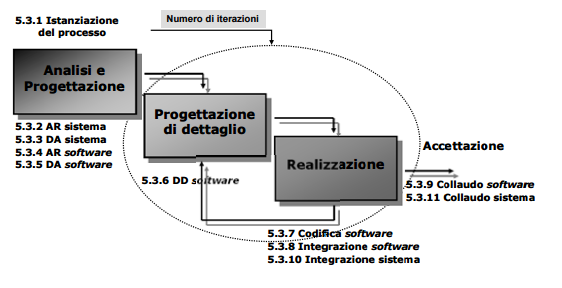
\includegraphics[width=0.75\columnwidth]{img4} % Example image
	\\Non ritorno mai sul progetto generale.\\
	
	\item \textbf{Iterativo:} comporta il rischio di non convergenza all'obbiettivo, tuttavia consentono maggior capacità di adattamento. Ogni iterazione comporta un ritorno all'indietro, nella direzione opposta rispetto al tempo.
	\item \textbf{Evolutivo:} insegue il futuro non ritirando il passato, ho tante attività concorrenti.Questo modello lo attua chi può sostenere molte versioni in parallelo (e quindi ha buone capacità finanziarie), infatti ogni fase ammette iterazioni multiple e parallele. Si può anche modificare la base ATT.
	\item\textbf{Spirale:} è composto da cicli interni rapidi e ripetuti, mentre quelli esterni aderiscono a qualsiasi altro modello std. Comporta un miglior controllo dei rischi di progetto, infatti pone molta attenzione sugli aspetti gestionali (pianificazione delle fasi, analisi dei rischi), è un modello \textbf{risk driven}. Prevede 4 attività principali 				 		\begin{itemize}
			\item Definizione degli obbiettivi
			\item Analisi dei rischi
			\item Sviluppo e validazione
			\item Pianificazione
		\end{itemize}
	Utilizzato solo per progetti innovativi
		
		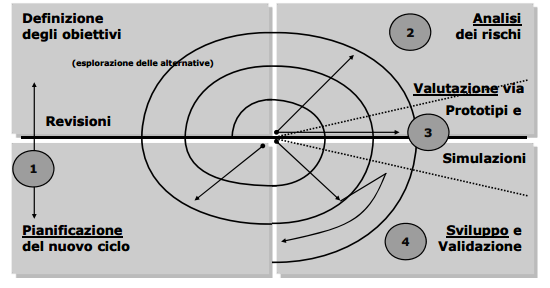
\includegraphics[width=0.75\columnwidth]{img5} % Example image
		\\
		I quadrati rappresentano dei macrostati.
		\item \textbf{Componenti:} si basa sul riuso dei componenti già fatti, utilizzo meno risorse ed ho un ecosistema(librerie e strumenti) già pronti.
\end{itemize}

\textbf{Metodi agili}, opposizione al modello sequenziale. 4 principi su cui si basa:

\begin{enumerate}

	\item Mettere in primo piano persone e iterazioni piuttosto che processi e strumenti. Gli individui sono importanti ed è importante il modo in cui interagiscono tra loro;
	
	\item "\textit{Dei documenti me ne frego, basta che funzioni}". La documentazione non sempre corrisponde a sw funzionante. E' importante che funzioni. Ma nel lungo periodo farà soffrire chi dovrà prendere in mano il sw;
	
	\item Avere un buon rapporto con il customer, coinvolgerlo, non ingessare il rapporto;
	
	\item Reattività piuttosto che pianificazione. Capacità di adattamento a cambiamenti delle situazioni.

\end{enumerate}

Il modello agile è maturato in qualcosa di plausibile, in alcune tecniche che funzionano.

\textbf{Modello agile educato}, tutto ruota intorno al "\textit{document user story}", è l'espressione precisa di quello che l'utente vuole in quel momento. Associato ad ogni user story produrre una strategia che sia in grado di soddisfare quei bisogni. User story associato a un insieme di cose da fare che dimostrino al customer che c'è una soluzione (\textbf{product backlog}). Quello che si ottiene va verso il customer o in feedback. C'è un supervisore che decide l'urgenza strategica (\textbf{sprint}). Tutti fanno un pezzo e poi lo consegnano. Ogni iterazione è rapida e va molto verso le aspettative del cliente.

\textbf{Scrum daily}, mucchio giornaliero, un contatto giornaliero dell'avanzamento. Tecnica ragionevole per chi ha poca esperienza.

\end{document}